\documentclass[tikz,border=2pt]{standalone}
\usepackage{amsmath}
\usetikzlibrary{arrows.meta,decorations.pathreplacing}
\begin{document}
% Single-item inventory system at the start of period 4 of the (s,S) = (3,8), l = 1 example:
% P'_3 = 3 <= s triggers Q_4 = 5 (in transit), on-hand stock I_4 = 3 meets demand D_4 = 2,
% inventory level I_4 = 3 and inventory position P_4 = I_4 + Q_4 = 8.
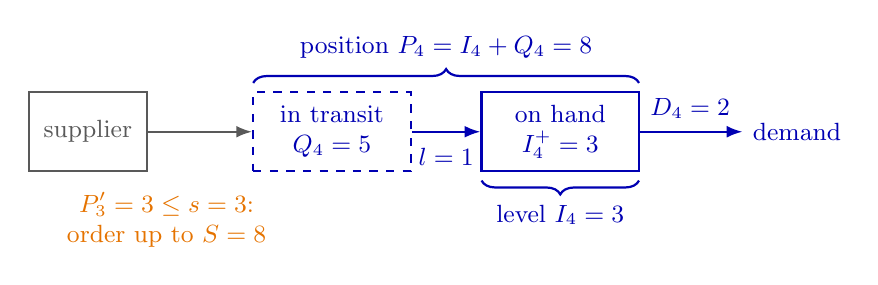
\begin{tikzpicture}[font=\small, >={Latex[length=2mm]},
    box/.style={draw, thick, minimum height=1.0cm, align=center, inner sep=3pt}]
  \node[box, gray!70!black, minimum width=1.5cm] (sup) at (0,0) {supplier};
  \node[box, blue!70!black, dashed, minimum width=2.0cm] (tr) at (3.1,0) {in transit\\$Q_4=5$};
  \node[box, blue!70!black, minimum width=2.0cm] (sh) at (6.0,0) {on hand\\$I_4^+=3$};
  \draw[->, thick, gray!70!black] (sup.east) -- (tr.west);
  \draw[->, thick, blue!70!black] (tr.east) -- (sh.west);
  \draw[->, thick, blue!70!black] (sh.east) -- ++(1.3,0) node[anchor=west] {demand};
  \node[blue!70!black, anchor=south] at (7.65,0.05) {$D_4=2$};
  \node[blue!70!black, anchor=north] at (4.55,-0.08) {$l=1$};
  % policy decision
  \node[orange!90!black, anchor=north, align=center] at (1.0,-0.65) {$P'_3=3\le s=3$:\\order up to $S=8$};
  % braces
  \draw[decorate, decoration={brace, amplitude=5pt}, thick, blue!70!black]
    (2.1,0.62) -- (7.0,0.62) node[midway, anchor=south, yshift=5pt] {position $P_4=I_4+Q_4=8$};
  \draw[decorate, decoration={brace, amplitude=5pt, mirror}, thick, blue!70!black]
    (5.0,-0.62) -- (7.0,-0.62) node[midway, anchor=north, yshift=-5pt] {level $I_4=3$};
\end{tikzpicture}
\end{document}
